
% This LaTeX was auto-generated from an M-file by MATLAB.
% To make changes, update the M-file and republish this document.

\documentclass{article}
\usepackage{graphicx}
\usepackage{color}
\usepackage{listings}
\usepackage[framed]{mcode}
\usepackage{fullpage}
\usepackage{amsmath}
\usepackage[utf8x]{inputenc}
\usepackage{import}
\usepackage{setspace}
\usepackage{hyperref}
\definecolor{lightgray}{gray}{0.5}
\setlength{\parindent}{0pt}

\begin{document}

    
    
%\section*{}


\title{BE 521: Homework 3 Questions\\{\normalsize Feature extraction} \\{\normalsize Spring 2021}}
\author{68 points}
\date{Due: Tuesday, 2/16/2021 10pm}
\maketitle
\textbf{Objective:} Extract features from data and build a simple detector


\begin{center}
\author{Jal Mahendra Panchal \\
  \normalsize Collaborators: COLLABORATORS HERE \\}
\end{center}


\section{Features and Simulations (39 pts)} As you learned
in class, features are the backbone of almost all detection
strategies, from seizures in EEG to faces in images. Features are
usually defined in journal articles as an equation or set of
equations, and the task for the reader---if she wants to use that
feature---is to implement that feature in code. In this section, you
will explore and implement some features commonly used in EEG
analysis and test them on simulated time-series data.
\begin{enumerate}
 \item Consider the following toy signal: 7 seconds of a 2 Hz sine
 wave with a quarter period phase-shift, sampled at 100 Hz
  \begin{enumerate}
   \item Plot the signal. (2 pts)



\subsection*{Answer P1 Q1(a)}


\\ Answer : \\

Signal characteristics :
\begin{lstlisting}
duration_s = 7;
signal_frequency_hz = 2;
sampling_frequency_hz = 100;
theta_rad =  pi/2;
t = 0: 1/sampling_frequency_hz : duration_s-1/sampling_frequency_hz;

sine_wave = sin(2*pi*signal_frequency_hz*t + theta_rad);
\end{lstlisting}
Plot
\begin{lstlisting}
figure();
plot(t, sine_wave, 'Linewidth', 1);
title('Sine Wave')
xlabel('Time (s)')
ylabel('Amplitude')
ylim ([-1.5,1.5])
\end{lstlisting}


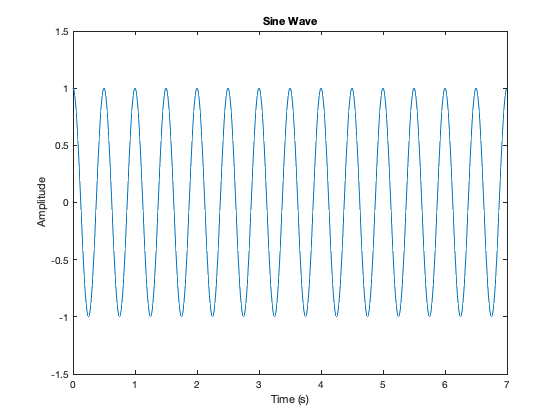
\includegraphics [width=5in]{jalp_hw3_01.png}

\item Using the Matlab functions for the difference, sum, and
  absolute value of the elements in a vector (look them up if you
  don't know them), create an anonymous function for the
   line-length feature
	$ LL(\mathbf{x}) = \sum_{i=2}^{n} |x_i - x_{i-1}| $ in one line of
	Matlab code that uses no loops (i.e., the outputs of one function
	will be the inputs of another). Your function should look
	something like \begin{lstlisting}
	  LLFn = @(x) XXXXXX;
	\end{lstlisting}
	where \texttt{XXXXX} represents some use of the aformentioned functions and the input signal \texttt{x}. (4 pts)



\subsection*{Answer P1 Q1(b)}


\\ Answer : \\



\subsection*{Line Length function}

We will define an anonymous funtionn to calculate line length
\begin{lstlisting}
LLFn = @(x) sum(abs(diff(x)));
\end{lstlisting}

   \item What is the line length of this signal? (2 pts)
  \end{enumerate}



\subsection*{Answer P1 Q1(c)}


\\ Answer : \\

\begin{lstlisting}
%Calling the LLFn function
line_length = LLFn(sine_wave)
\end{lstlisting}

\color{lightgray} \begin{lstlisting}
line_length =

   55.9921

\end{lstlisting} \color{black}

The line length of the sine wave is 55.9921 units.


 \item Consider line length of the signal using a sliding window
 with a certain amount of window overlap (or, to think of it another
 way, displacement with each ``slide''). Now, instead of having just
 one value for the line length, you will have a number of values.
  \begin{enumerate}
	\item Given a signal \texttt{x} with sampling frequency
	\texttt{fs} and windows of length \texttt{winLen} and displacement
	\texttt{winDisp} (both in seconds), create an anonymous function
	called \texttt{NumWins} that calculates the number of possible
	(full) windows in your signal of length \texttt{xLen} (in
	samples), i.e., \begin{lstlisting}
	  NumWins = @(xLen, fs, winLen, winDisp) XXXXXX;
	\end{lstlisting} where \texttt{XXXXXX} is the single-line
	expression for this value. You may assume that \texttt{winDisp} is
	a factor of both \texttt{winLen} (as it usually is/should be)
	and the length (in seconds) of \texttt{x}. (4 pts)



\subsection*{Answer P1 Q2(a)}


\\ Answer : \\



\subsection*{Number of windows function}

\begin{lstlisting}
%The number of windows can be found using the following function
NumWins = @(xLen, fs, winLen, winDisp) floor((xLen-(winLen-winDisp))/(winDisp));
\end{lstlisting}

  \item Use this
	function to calculate the number of windows for the signal
	described in Question 1.1 for a 400 ms window with 200 ms
	displacement, i.e., the expression \begin{lstlisting}
	  NumWins(length(x), fs, winLen, winDisp)
	\end{lstlisting}
	where \texttt{fs}, \texttt{winLen}, and \texttt{winDisp} are the appropriate values. (1 pt)



\subsection*{Answer P1 Q2(b)}


\\ Answer : \\

\begin{lstlisting}
duration_ms = 7000;
win_len_ms = 400;
win_disp_ms = 200;
NumberOfWindows_2_1 = NumWins(duration_ms, sampling_frequency_hz, win_len_ms, win_disp_ms)
\end{lstlisting}

\color{lightgray} \begin{lstlisting}
NumberOfWindows_2_1 =

    34

\end{lstlisting} \color{black}

The number of windows of length 400ms and displacement 200ms in a 7s signal are 34;


	\item Repeat the above calculation for 50 ms window displacement. (1 pt)



\subsection*{Answer P1 Q2(c)}


\\ Answer : \\

\begin{lstlisting}
duration_ms = 7000;
win_len_ms = 400;
win_disp_ms = 50;
NumberOfWindows_2_2 = NumWins(duration_ms, sampling_frequency_hz, win_len_ms, win_disp_ms)
\end{lstlisting}

\color{lightgray} \begin{lstlisting}
NumberOfWindows_2_2 =

   133

\end{lstlisting} \color{black}

The number of windows of length 400ms and displacement 50ms in a 7s signal are 133;


	\item Repeat the above calculation for 100 ms window displacement. (1 pt)
  \end{enumerate}



\subsection*{Answer P1 Q2(d)}


\\ Answer : \\

\begin{lstlisting}
duration_ms = 7000;
win_len_ms = 400;
win_disp_ms = 100;
NumberOfWindows_2_3 = NumWins(duration_ms, sampling_frequency_hz, win_len_ms, win_disp_ms)
\end{lstlisting}

\color{lightgray} \begin{lstlisting}
NumberOfWindows_2_3 =

    67

\end{lstlisting} \color{black}

The number of windows of length 400ms and displacement 100ms in a 7s signal are 67;


  \item
  \begin{enumerate}
   \item Create a function (in another file) called
   \texttt{MovingWinFeats(x, fs, winLen, winDisp, featFn)} that
   returns a vector of the values of the feature on the signal
   \texttt{x} in all the possible windows, where \texttt{featFn} is
   a feature function like the one you wrote in Question 1.1.b. You
   may find it useful to use your \texttt{NumWins} function (or at
   least its expression). You may assume that the product of
   \texttt{winDisp} and the sampling rate \texttt{fs} is an integer.
   (6 pts) \\


Make sure your MovingWinFeats code is in your pdf. One way is to use the following Matlab code (in your script) to automatically
load in the function's code (where we assume that the function is
one directory up from the *.tex file). Windows users may need to
change the forward-slash to a backslash.

\begin{lstlisting}
%   <latex>
%   \lstinputlisting{[path to] MovingWinFeats.m}
%   </latex>
\end{lstlisting}


\subsection*{Answer P1 Q3(a)}


\\ Answer : \\
\lstinputlisting{MovingWinFeats.m}


   \item Using the signal you defined in Question 1.1 and the function you created in Question 1.1.b, calculate the line-length over windows of length 400 ms and displacement 200 ms. (2 pts)



\subsection*{Answer P1 Q3(b)}


\\ Answer : \\

Using function MovingWinFeats to calculate Line Length
\begin{lstlisting}
x = sine_wave;
fs = sampling_frequency_hz;
winLen = 400 ; %in ms
winDisp = 200; %in ms
line_length_windows_3c = MovingWinFeats(x, fs, winLen, winDisp, LLFn);
\end{lstlisting}
\begin{lstlisting}
%Plotting linelength for each window
figure();
plot(line_length_windows_3c, 'o-')
title('Line Length for 400 ms winLen, 200 winDisp')
xlabel('window index')
ylabel('line length amplitude')
\end{lstlisting}


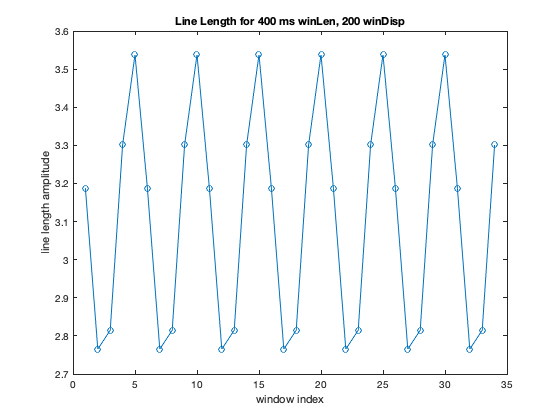
\includegraphics [width=5in]{jalp_hw3_02.png}

   \item Add a unit-amplitude 10 Hz signal (in the form of a sine wave) to your original signal and again calculate the line length over the same window and displacement. (2 pts)
  \end{enumerate}



\subsection*{Answer P1 Q3(c)}


\\ Answer : \\

\begin{lstlisting}
%Adding a 10 Hz signal
duration_s = 7;
signal_frequency_hz = 10;
sampling_frequency_hz = 100;
t = 0: 1/sampling_frequency_hz : duration_s-1/sampling_frequency_hz;
sine_wave_10 = sin(2*pi*10*t);

sine_wave_cmb = sine_wave + sine_wave_10;

% Using function MovingWinFeats to calculate Line Length
x = sine_wave_cmb;
fs = sampling_frequency_hz;
winLen = 400 ; %in ms
winDisp = 200; %in ms
line_length_windows_3d = MovingWinFeats(x, fs, winLen, winDisp, LLFn);
\end{lstlisting}

  \item Code the following 3 additional features in MINIMAL lines of code (hint: each can be implemented in one line using the anonymous function trick).
  \begin{enumerate}
   \item Area, $\displaystyle A(\mathbf{x}) = \sum_{i=1}^{n} |x_i| $ \quad (2 pts)



\subsection*{Answer P1 Q4(a)}


\\ Answer : \\

\begin{lstlisting}
AreaFn = @(x) sum(abs(x));
\end{lstlisting}

   \item Energy, $\displaystyle E(\mathbf{x}) = \sum_{i=1}^{n} x_i^2 $ \quad (2 pts)



\subsection*{Answer P1 Q4(b)}


\\ Answer : \\

\begin{lstlisting}
EnergyFn = @(x) sum(x.^2);
\end{lstlisting}

   \item Zero-Crossings around mean,\\ $\displaystyle ZX(\mathbf{x}) = \sum_{i=2}^{n} \mathbf{1}(\mathbf{FromAbove}) \;\mbox{OR}\; \mathbf{1}(\mathbf{FromBelow})$,
       where $\mathbf{1}(\cdot)$ denotes the indicator function, which returns a zero if its argument is false and a one if it is true,
       $\mathbf{FromAbove}$ denotes $(x_{i-1} - \overline{x} > 0) \;\mbox{AND}\; (x_i - \overline{x} < 0)$,
       $\mathbf{FromBelow}$ denotes $(x_{i-1} - \overline{x} < 0) \;\mbox{AND}\; (x_i - \overline{x} > 0)$,
       and $\overline{x}$ is the mean value of the elements in $x$. (4 pts)



\subsection*{Answer P1 Q4(c)}


\\ Answer : \\

Here we first remove the mean from the signal Then we find values above and below the mean We then calculate the difference between the signs of consecutive values if the absolute value of this difference is \ensuremath{>} 2 then its a zero crossing We then find the number of indices where zero crossing occcurs.
\begin{lstlisting}
ZeroCrossingFn = @(x) size(find(abs(diff(sign(x-mean(x))))>1),2);
\end{lstlisting}

   \item Plot the values of the four features on the combined signal in the first four cells of a 3x2 matlab subplot.
   Use a 400 ms window with 100 ms displacement. Using the right-aligned convention (where the
   ``official'' time of the feature is that of the last data point
   in the window), give the appropriate time axis for each window
   point. In addition, plot the original signal with the 2Hz and 10Hz
   components in the last two cells of the 3x2 subplot (to make
   comparing down the column easy). Ensure that the time axis in all
   of your plots is the same. (6 pts)



\subsection*{Answer P1 Q4(d)}


\\ Answer : \\



\subsection*{Computing values 4(d)}

\begin{lstlisting}
x = sine_wave_cmb;
fs = sampling_frequency_hz;
winLen = 400 ; %in ms
winDisp = 100; %in ms

[line_length_windows_4d, ni, win_start, win_end] = MovingWinFeats(x, fs, winLen, winDisp, LLFn);
area_4d = MovingWinFeats(x, fs, winLen, winDisp, AreaFn);
energy_4d = MovingWinFeats(x, fs, winLen, winDisp, EnergyFn);
zero_crossing_4d = MovingWinFeats(x, fs, winLen, winDisp, ZeroCrossingFn);
\end{lstlisting}


\subsection*{Plotting the graph 4(d)}

\begin{lstlisting}
t = 0: 1/sampling_frequency_hz : duration_s-1/sampling_frequency_hz;
t_win_end = t(ni+win_end);

figure();
subplot(3,2,1)
plot(t_win_end, line_length_windows_4d, 'o-', 'Linewidth', 1, 'Color',[0, 0.4470, 0.7410])
title('Line Length in window')
xlabel('Time (s)')
ylabel('line length amplitude')
ylim([0.995*min(line_length_windows_4d), 1.005*max(line_length_windows_4d)])

subplot(3,2,2)
plot(t_win_end, area_4d, 'o-', 'Linewidth', 1, 'Color', [0.8500, 0.3250, 0.0980])
title('Area in window')
xlabel('Time (s)')
ylabel('Area amplitude')
ylim([0.9*min(area_4d), 1.1*max(area_4d)])

subplot(3,2,3)
plot(t_win_end, energy_4d, 'o-', 'Linewidth', 1, 'Color', [0.4660, 0.6740, 0.1880])
title('Energy in window')
xlabel('Time (s)')
ylabel('Energy amplitude')
ylim([0.9*min(energy_4d), 1.1*max(energy_4d)])


subplot(3,2,4)
plot(t_win_end, zero_crossing_4d, 'o-', 'Linewidth', 1, 'Color', [0.9290, 0.6940, 0.1250])
title('Total Zero crossings in window')
xlabel('Time (s)')
ylabel('Number of Zero Crossings')
ylim([0.9*min(zero_crossing_4d), 1.1*max(zero_crossing_4d)])


subplot(3,2,5)
plot(t, x , 'Linewidth', 1)
title('Signal')
xlabel('Time (s)')
ylabel('Signal amplitude')
ylim([1.1*min(x), 1.1*max(x)])


subplot(3,2,6)
plot(t, x , 'Linewidth', 1)
title('Signal')
xlabel('Time (s)')
ylabel('Signal amplitude')
ylim([1.1*min(x), 1.1*max(x)])


suptitle('Features in window : 400 ms WinLen, 100ms WinDisp')
\end{lstlisting}


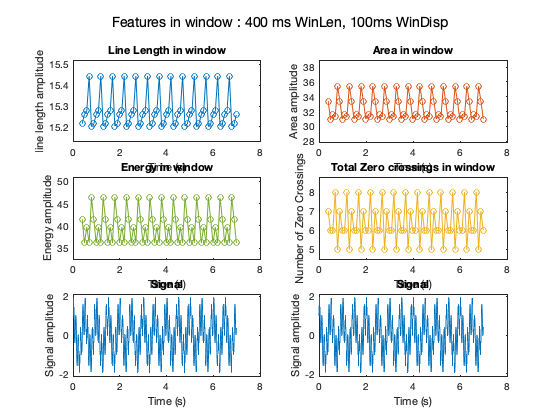
\includegraphics [width=5in]{jalp_hw3_03.png}

  \end{enumerate}
\end{enumerate}
\section{Feature Overlays (17 pts)}
In this section, you will use a line-length feature overlay on a segment of EEG containing a seizure. This data is stored in \texttt{I521\_A0003\_D001}
\begin{enumerate}
 \item What is the length using hours:minutes:seconds:milliseconds of the recording? (Use getDuration) (2 pts)



\subsection*{Answer P2 Q1}


\\ Answer : \\



\subsection*{Fetching signal}

\begin{lstlisting}
addpath(genpath('/Users/jalpanchal/git/be521'));

session_sez = IEEGSession('I521_A0003_D001', 'jalpanchal', 'jal_ieeglogin.bin');
sampling_frequency_hz_sez = session_sez.data.sampleRate;
duration_in_sec_sez = session_sez.data(1).rawChannels(1).get_tsdetails.getDuration/1e6;

sez_data = session_sez.data.getvalues(0, duration_in_sec_sez * 1e6, 1);
\end{lstlisting}

\color{lightgray} \begin{lstlisting}IEEGSETUP: Adding 'ieeg-matlab.jar' to dynamic classpath
IEEGSETUP: Found log4j on Java classpath.
URL: https://www.ieeg.org/services
Client user: jalpanchal
Client password: ****
\end{lstlisting} \color{black}
\begin{lstlisting}
datestr(seconds(duration_in_sec_sez),'HH:MM:SS:FFF')
\end{lstlisting}

\color{lightgray} \begin{lstlisting}
ans =

    '01:21:20:390'

\end{lstlisting} \color{black}

The duration of the signal I521\_A0003\_D001 in
hours:minutes:seconds:milliseconds is 01:21:20:390.\\


 \item How many data points should we discard at the end if we want to clip the recording to the last full second? Do this clipping. (1 pt)



\subsection*{Answer P2 Q2}


\\ Answer : \\
The signal has 390ms of data which needs to be discarded. At 200 Hz and
5ms between every sample, we will have to discard the last 78 data
points. \\

Discarding the last 78 data points
\begin{lstlisting}
sez_data_trim = sez_data(1:end-78);
\end{lstlisting}

 \item If we want to overlay a feature trace on the original signal, we have to interpolate that feature (which has been calculated over windows) for each data point of the original signal. One of the simplest methods of doing this is called zero-order interpolation, where we just hold the value constant until we get to the next calculated value. For example, if we had a moving window of 1 second with 1 second displacement, the zero-order interpolated feature vector would have the same value the entire first second, then the same for the entire second second, etc, where each second contains the same number of points as the sampling frequency of the original signal.
 \begin{enumerate}
  \item Using the \texttt{repmat} and \texttt{reshape} functions, create an external function \texttt{zoInterp(x, numInterp} that copies each value of \texttt{x} \texttt{numInterp} times. You can implement this function in one line of code with no loops. Include the code for this function as you did in Question 1.3.a. (2 pts)



\subsection*{Answer P2 Q3(a)}


\\ Answer : \\
\lstinputlisting{zoInterp.m}


  \item Confirm that this function works correctly by expanding the length of the vector \texttt{1:5} by a factor of 5 and plotting with the command
  \begin{lstlisting}
	plot(zoInterp(1:5,5),'-o')
  \end{lstlisting}
  where the \texttt{'-o'} option lets us see the individul points as well as the line that connects them. (2 pts)
 \end{enumerate}



\subsection*{Answer P2 Q3(b)}


\\ Answer : \\

\begin{lstlisting}
figure();
plot(zoInterp(1:5,5), '-o')
title('Example of zoInterp')
xlabel('Signal index')
ylabel('Signal amplitude')
\end{lstlisting}


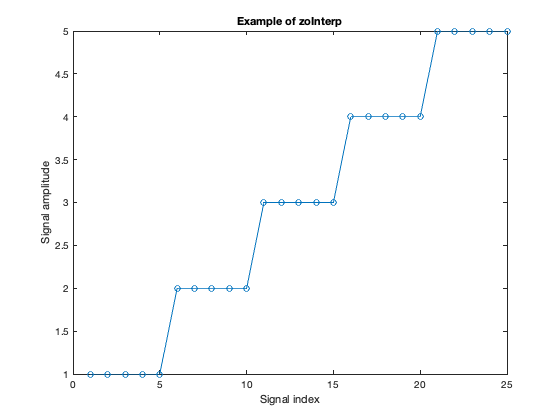
\includegraphics [width=5in]{jalp_hw3_04.png}

 \item Using a 5-second sliding window with 1-second displacement,
 calculate the line length feature over the entire signal. Normalize
 the line-length feature values to have a maximum twice that of the
 original EEG signal maximum. Plot the signal in blue and overlay
 the right-aligned line-length feature in yellow. Note: you will need
 to pad your
 signal in order to get them to line up correctly and be the
 same length. Put the units of your time axis in minutes, and be
 sure to add a legend in a location in the plot that does not cover
 up any signal or feature. (6 pts)



\subsection*{Answer P2 Q4}


\\ Answer : \\

\begin{lstlisting}
%Calcualting Line Length for I521_A0003_D001
x = sez_data_trim';
fs = sampling_frequency_hz_sez;
winLen_ms = 5000; %in ms
winDisp_ms = 1000; %in ms
[line_length_sez, ni_sez, win_st_sez, win_end_sez] = MovingWinFeats(x, fs, winLen_ms, winDisp_ms, LLFn);

%Scaling line length to have a max value = 2x max of signal
scaling_factor = 2*max(sez_data_trim)/max(line_length_sez);

%Normalizing line length
line_length_norm = scaling_factor*line_length_sez;

%padding Linelength
ni = ni_sez*1e-3*fs; % ni in number of samples
L = winLen_ms*1e-3*fs; % L in number of samples
d = winDisp_ms*1e-3*fs; % d in number of samples

line_length_pad = [NaN(1,ni+L-1) zoInterp(line_length_norm(1:end-1),d) line_length_norm(end)];
\end{lstlisting}
\begin{lstlisting}
%Plotting
figure();
len_s = size(sez_data_trim,1)/fs;
t = (0:1/fs : len_s-1/fs)/60;
plot(t, sez_data_trim,'Linewidth', 0.1, 'Color', [0, 0.4470, 0.7410]);
hold on
plot(t, line_length_pad, 'Linewidth', 1, 'Color', [0.8500, 0.3250, 0.0980])
hold off
title('Normalized Line Length overlay on EEG for I521\_A0003\_D001')
xlabel('Time (min)')
ylabel('Signal Amplitude (\muV)')
xlim([-1,82])
legend('EEG signal', 'Normalized Line Length')
\end{lstlisting}


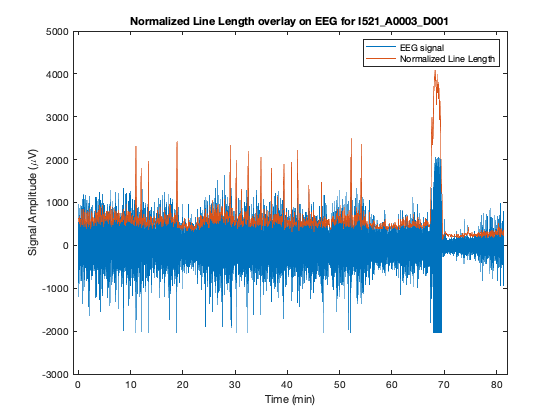
\includegraphics [width=5in]{jalp_hw3_05.png}

 \item What threshold might you use on the raw line-length feature
 vector (not the normalized one used for plotting) in order to
 capture the 17 largest pre-seizure chirps that occur? (1 pt)



\subsection*{Answer P2 Q5}


\\ Answer : \\
We can select the threshold visually to detect 17 peaks.

\begin{lstlisting}
%Verification of threshold
line_length_raw_pad = [NaN(1,ni+L-1) zoInterp(line_length_sez(1:end-1),d) line_length_sez(end)];
%only considering pre-seizure signal
line_length_raw_presz = line_length_raw_pad(1:end-20*60*200);

%Peaks found with threshold
x = line_length_raw_presz;
threshold = 4.3*1e4;
y = x>threshold;
peaks_found = size(find(diff(sign(y))==1),2)
\end{lstlisting}

\color{lightgray} \begin{lstlisting}
peaks_found =

    17

\end{lstlisting} \color{black}
\begin{lstlisting}
%Finding threshold for 17 pre seizure peaks
% plot the threshold on EEG signal
figure();
t = (0:1/fs : len_s-1/fs)/60;
plot(t(1:end-20*60*200), line_length_raw_presz, 'Linewidth', 1, 'Color', [0.8500, 0.3250, 0.0980])
hold on
yline(threshold, 'Linewidth', 2, 'Color', [0 0 0])
hold off
title('Finding threshold from Line Length from pre-seizure 17 peaks')
xlabel('Time (min)')
ylabel('Line length units')
legend('Line Length','Threshold')
xlim([0,62])
\end{lstlisting}


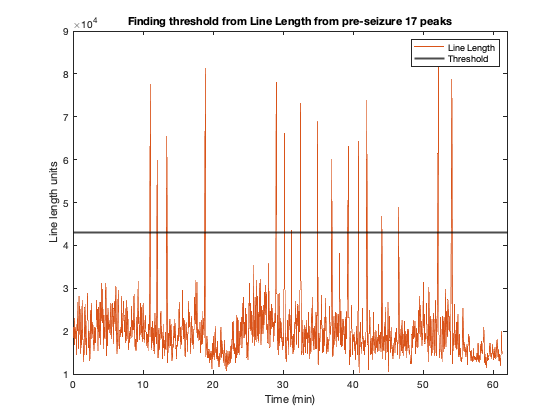
\includegraphics [width=5in]{jalp_hw3_06.png}

 \item Using this threshold value, in another plot draw red vertical lines at the leading point in time where the threshold is crossed. Add these vertical lines on top of the plot you made in Question 2.4. These events should capture the pre-seizure chirps, the seizure onset, and some flickering during the end of the seizure. (3 pts)



\subsection*{Answer P2 Q6}


\\ Answer : \\

Finding the index energy signal when it crosses threshold
\begin{lstlisting}
x = line_length_raw_pad;
threshold = 4.3*1e4;
y = x>threshold;
crossing_index = find(diff(sign(y))==1);
crossing_index = crossing_index/fs/60; %in mins
\end{lstlisting}
\begin{lstlisting}
%Plotting
figure();
len_s = size(sez_data_trim,1)/fs;
t = (0:1/fs : len_s-1/fs)/60;
plot(t, sez_data_trim,'Linewidth', 0.1, 'Color', [0, 0.4470, 0.7410]);
hold on
plot(t, line_length_pad, 'Linewidth', 1, 'Color', [0.8500, 0.3250, 0.0980])
for i=crossing_index
    xline(i, 'Linewidth', 1)
end
hold off
title('Normalized Line Length overlay on EEG for I521\_A0003\_D001')
xlabel('Time (min)')
ylabel('Signal Amplitude (\muV)')
xlim([-1,82])
legend('EEG signal', 'Normalized Line Length', 'Threshold Crossing')
\end{lstlisting}


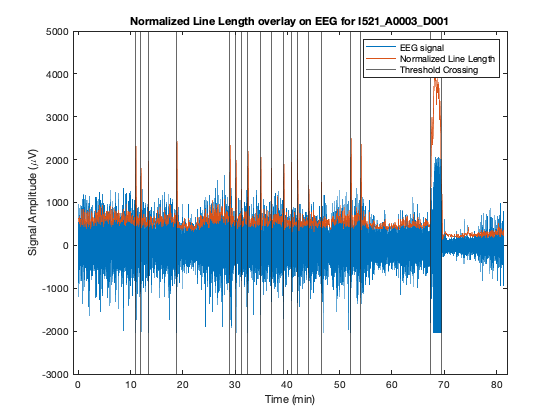
\includegraphics [width=5in]{jalp_hw3_07.png}

\end{enumerate}
\section{Building a Detector (12 pts)}
In this section, you will use the features you defined previously to build a seizure detector. Use the EEG data in the file \texttt{I521\_A0003\_D002} with channels \texttt{multiSz\_1}, and \texttt{multiSz\_2}.
\begin{enumerate}
 \item Plot the signal in \texttt{multiSz\_1} and draw vertical red lines at the times when you think the two seizures begin. (You should be able to do this without the need of any features.) (2 pts)



\subsection*{Answer P3 Q1}


\\ Answer : \\



\subsection*{Fetching signal}

\begin{lstlisting}
session_mulsez = IEEGSession('I521_A0003_D002', 'jalpanchal', 'jal_ieeglogin.bin');
sampling_frequency_hz_mulsez = session_mulsez.data.sampleRate;
duration_in_sec_mulsez = session_mulsez.data(1).rawChannels(1).get_tsdetails.getDuration/1e6;

multisz_1 = session_mulsez.data.getvalues(0, duration_in_sec_mulsez * 1e6, 1);
multisz_2 = session_mulsez.data.getvalues(0, duration_in_sec_mulsez * 1e6, 2);

datestr(seconds(duration_in_sec_mulsez),'HH:MM:SS:FFF')
\end{lstlisting}

\color{lightgray} \begin{lstlisting}IEEGSETUP: Adding 'ieeg-matlab.jar' to dynamic classpath
Warning: Objects of edu/upenn/cis/db/mefview/services/TimeSeriesDetails
class exist - not clearing java 
Warning: Objects of edu/upenn/cis/db/mefview/services/TimeSeriesInterface
class exist - not clearing java 
IEEGSETUP: Found log4j on Java classpath.
URL: https://www.ieeg.org/services
Client user: jalpanchal
Client password: ****

ans =

    '04:09:59:995'

\end{lstlisting} \color{black}
\begin{lstlisting}
len_s = duration_in_sec_mulsez;
fs = sampling_frequency_hz_mulsez;
t = (0:1/fs : len_s-1/fs)/60;

%Index for start of 2 seizures, selected from visual inspection
sez_1_indx = 8;
sez_2_indx = 151;

figure();
plot(t, multisz_1,'Linewidth', 0.1, 'Color', [0, 0.4470, 0.7410]);
hold on
xline(sez_1_indx, 'Linewidth', 1.5, 'Color', 'r');
xline(sez_2_indx, 'Linewidth', 1.5, 'Color', 'r');
hold off
title('Seizure indicators for I521\_A0003\_D002')
xlabel('Time (min)')
ylabel('Signal Amplitude (\muV)')
\end{lstlisting}


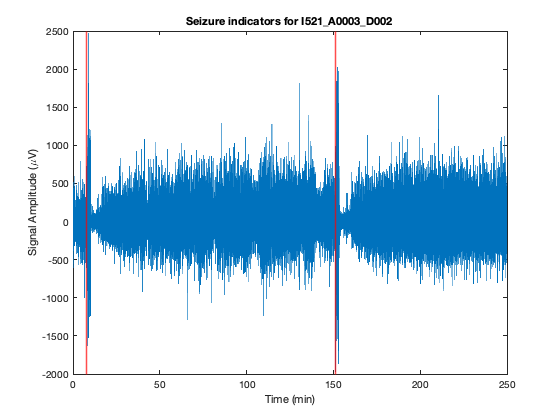
\includegraphics [width=5in]{jalp_hw3_08.png}

 \item Produce feature overlay plots similar to that of Question 2.4 for each of the four features you have implemented along with the red vertical lines at each seizure. Use the same 4-second sliding window with 1 second displacement. (4 pts)



\subsection*{Answer P3 Q2}


\\ Answer : \\



\subsection*{Computing values 4(d)}

\begin{lstlisting}
x = multisz_1';
fs = sampling_frequency_hz_mulsez;
winLen = 4000 ; %in ms
winDisp = 1000; %in ms

[line_length_ms1, ni_ms, win_start_ms, win_end_ms] = MovingWinFeats(x, fs, winLen, winDisp, LLFn);
area_ms1 = MovingWinFeats(x, fs, winLen, winDisp, AreaFn);
energy_ms1 = MovingWinFeats(x, fs, winLen, winDisp, EnergyFn);
zero_crossing_ms1 = MovingWinFeats(x, fs, winLen, winDisp, ZeroCrossingFn);
\end{lstlisting}


\subsection*{Normalising features}

\begin{lstlisting}
scaling_factor = 2*max(multisz_1)/max(line_length_ms1);
line_length_norm_ms1 = scaling_factor*line_length_ms1;

scaling_factor = 2*max(multisz_1)/max(area_ms1);
area_norm_ms1 = scaling_factor*area_ms1;

scaling_factor = 2*max(multisz_1)/max(energy_ms1);
energy_norm_ms1 = scaling_factor*energy_ms1;

scaling_factor = 2*max(multisz_1)/max(zero_crossing_ms1);
zero_crossing_norm_ms1 = scaling_factor*zero_crossing_ms1;
\end{lstlisting}


\subsection*{Padding features}

\begin{lstlisting}
ni = ni_ms*1e-3*fs; % ni in number of samples
L = winLen*1e-3*fs; % L in number of samples
d = winDisp*1e-3*fs; % d in number of samples

line_length_pad_ms1 = [NaN(1,ni+L-1) zoInterp(line_length_norm_ms1(1:end-1),d) line_length_norm_ms1(end)];
area_pad_ms1 = [NaN(1,ni+L-1) zoInterp(area_norm_ms1(1:end-1),d) area_norm_ms1(end)];
energy_pad_ms1 = [NaN(1,ni+L-1) zoInterp(energy_norm_ms1(1:end-1),d) energy_norm_ms1(end)];
zero_crossing_pad_ms1 = [NaN(1,ni+L-1) zoInterp(zero_crossing_norm_ms1(1:end-1),d) zero_crossing_norm_ms1(end)];
\end{lstlisting}


\subsection*{Plotting the graphs}



\subsection*{Line length}

\begin{lstlisting}
figure();
len_s = size(multisz_1,1)/fs;
t = (0:1/fs : len_s-1/fs)/60;
plot(t, multisz_1,'Linewidth', 0.1, 'Color', [0, 0.4470, 0.7410]);
hold on
plot(t, line_length_pad_ms1, 'Linewidth', 1, 'Color', [0.8500, 0.3250, 0.0980])
xline(sez_1_indx, 'Linewidth', 2, 'Color', [0.4660, 0.6740, 0.1880]);
xline(sez_2_indx, 'Linewidth', 2, 'Color', [0.4660, 0.6740, 0.1880]);
hold off
title('Normalized Line Length overlay on EEG for I521\_A0003\_D002, multisz 1 channel')
xlabel('Time (min)')
ylabel('Signal Amplitude (\muV)')
legend('EEG signal', 'Normalized Line Length', 'Seizure indicator')
\end{lstlisting}


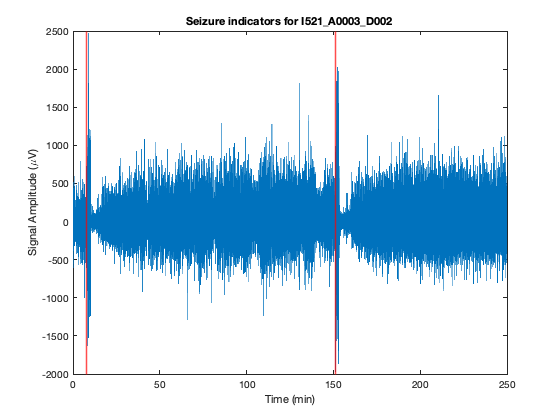
\includegraphics [width=5in]{jalp_hw3_09.png}


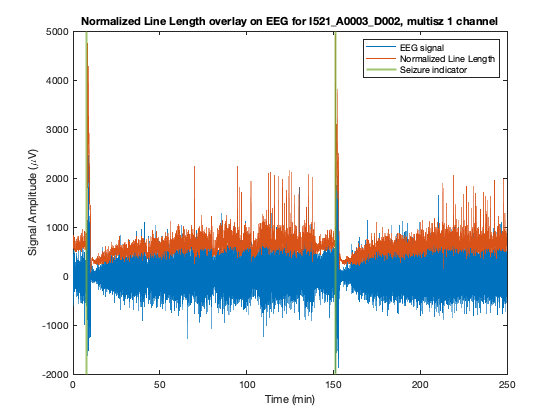
\includegraphics [width=5in]{jalp_hw3_10.png}


\subsection*{Area}

\begin{lstlisting}
figure();
len_s = size(multisz_1,1)/fs;
t = (0:1/fs : len_s-1/fs)/60;
plot(t, multisz_1,'Linewidth', 0.1, 'Color', [0, 0.4470, 0.7410]);
hold on
plot(t, area_pad_ms1, 'Linewidth', 1, 'Color', [0.8500, 0.3250, 0.0980])
xline(sez_1_indx, 'Linewidth', 2, 'Color', [0.4660, 0.6740, 0.1880]);
xline(sez_2_indx, 'Linewidth', 2, 'Color', [0.4660, 0.6740, 0.1880]);
hold off
title('Normalized Area overlay on EEG for I521\_A0003\_D002, multisz 1 channel')
xlabel('Time (min)')
ylabel('Signal Amplitude (\muV)')
legend('EEG signal', 'Normalized Area', 'Seizure indicator')
\end{lstlisting}


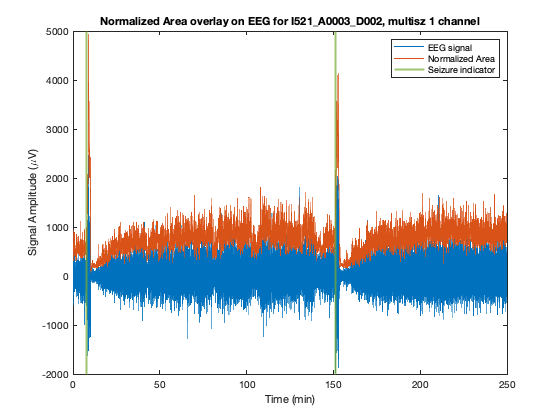
\includegraphics [width=5in]{jalp_hw3_11.png}


\subsection*{Energy}

\begin{lstlisting}
figure();
len_s = size(multisz_1,1)/fs;
t = (0:1/fs : len_s-1/fs)/60;
plot(t, multisz_1,'Linewidth', 0.1, 'Color', [0, 0.4470, 0.7410]);
hold on
plot(t, energy_pad_ms1, 'Linewidth', 1, 'Color', [0.8500, 0.3250, 0.0980])
xline(sez_1_indx, 'Linewidth', 2, 'Color', [0.4660, 0.6740, 0.1880]);
xline(sez_2_indx, 'Linewidth', 2, 'Color', [0.4660, 0.6740, 0.1880]);
hold off
title('Normalized Energy overlay on EEG for I521\_A0003\_D002, multisz 1 channel')
xlabel('Time (min)')
ylabel('Signal Amplitude (\muV)')
legend('EEG signal', 'Normalized energy', 'Seizure indicator')
\end{lstlisting}


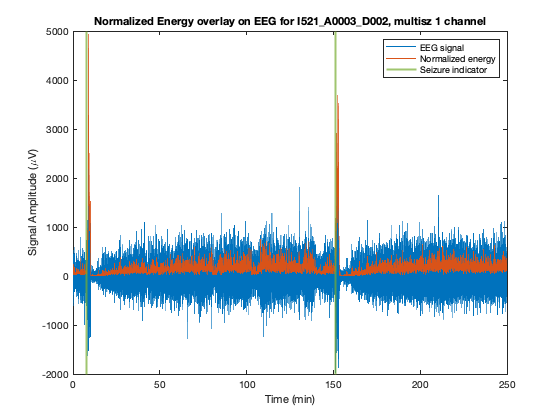
\includegraphics [width=5in]{jalp_hw3_12.png}


\subsection*{Zero Crossing}

\begin{lstlisting}
figure();
len_s = size(multisz_1,1)/fs;
t = (0:1/fs : len_s-1/fs)/60;
plot(t, multisz_1,'Linewidth', 0.1, 'Color', [0, 0.4470, 0.7410]);
hold on
plot(t, zero_crossing_pad_ms1, 'Linewidth', 1, 'Color', [0.8500, 0.3250, 0.0980])
xline(sez_1_indx, 'Linewidth', 2, 'Color', [0.4660, 0.6740, 0.1880]);
xline(sez_2_indx, 'Linewidth', 2, 'Color', [0.4660, 0.6740, 0.1880]);
hold off
title('Normalized Zero-Crossing overlay on EEG for I521\_A0003\_D002, multisz 1 channel')
xlabel('Time (min)')
ylabel('Signal Amplitude (\muV)')
legend('EEG signal', 'Normalized Zero-Crossing', 'Seizure indicator')
\end{lstlisting}


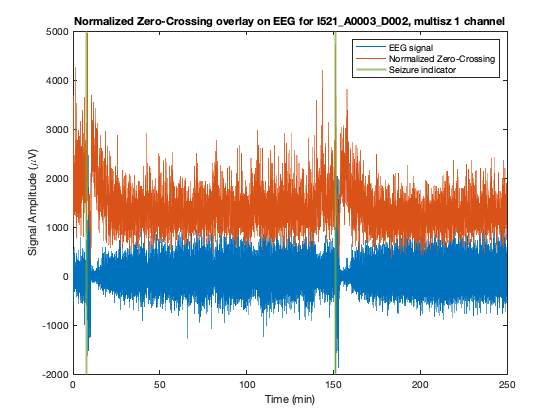
\includegraphics [width=5in]{jalp_hw3_13.png}

 \item
  \begin{enumerate}
   \item Based on your plots in the previous question, which of the
   four features seems to give the largest signal (relative to the
   background) for when a seizure occurs? Explain why you think this feature is the best. (3 pts)



\subsection*{Answer P3 Q3(a)}


\\ Answer : \\
To check which feature gives the largest signal as compared to
background, we will compute the ratio of $\frac{max value}{mean}$ for
each feature

\begin{lstlisting}
linelength_det_ratio = max(line_length_norm_ms1)/mean(line_length_norm_ms1)
area_det_ratio = max(area_norm_ms1)/mean(area_norm_ms1)
energy_det_ratio = max(energy_norm_ms1)/mean(energy_norm_ms1)
zerocrossing_det_ratio = max(zero_crossing_norm_ms1)/mean(zero_crossing_norm_ms1)
\end{lstlisting}

\color{lightgray} \begin{lstlisting}
linelength_det_ratio =

    7.5043


area_det_ratio =

    6.2745


energy_det_ratio =

   27.0870


zerocrossing_det_ratio =

    3.5446

\end{lstlisting} \color{black}

We get the ratio of $\frac{max value}{mean}$ as
\begin{enumeration}
\item Line Length = 7.5043
\item Area = 6.2745
\item Energy = 27.0870
\item Zero crossing = 3.5446. \\
\end{enumeration}
This is also confirmed through visual inspection of the graphs that the
Energy is the feature that is has the largest difference in
signal when a seizure occurs.\\
Seizures as Dr. Litt explained in the class tend to have a certain amount
of energy that needs to be dissipated forit to end. Having known this, it makes sense
if the energy plot shows the best indications of a seizure. As during a
seizure episode, the most amount of energy is dissipated in the form of the high
frequency signals we call "seizues", this is seen in the energy
signal as a big change from "normal"energy levels to high energy levels
of seizures.


   \item What threshold would you use to determine if a seizure is occurring? (1 pt)



\subsection*{Answer P3 Q3(b)}


\\ Answer : \\



\subsection*{Energy}

\begin{lstlisting}
figure();
len_s = size(multisz_1,1)/fs;
t = (0:1/fs : len_s-1/fs)/60;
threshold_energy = 1000;

plot(t, multisz_1,'Linewidth', 0.1, 'Color', [0, 0.4470, 0.7410]);
hold on
plot(t, energy_pad_ms1, 'Linewidth', 1, 'Color', [0.8500, 0.3250, 0.0980])
xline(sez_1_indx, 'Linewidth', 2, 'Color', [0.4660, 0.6740, 0.1880]);
xline(sez_2_indx, 'Linewidth', 2, 'Color', [0.4660, 0.6740, 0.1880]);
yline(threshold_energy, 'Linewidth', 2, 'Color', [0 0 0]);
hold off
title('Normalized Energy overlay on EEG for I521\_A0003\_D002, multisz 1 channel')
xlabel('Time (min)')
ylabel('Signal Amplitude (\muV)')
legend('EEG signal', 'Normalized energy', 'Seizure indicator', 'Energy threshold')
\end{lstlisting}


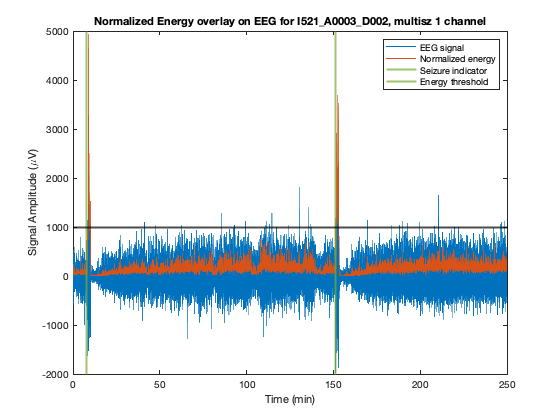
\includegraphics [width=5in]{jalp_hw3_14.png}
\begin{lstlisting}
%Non-normalized energy
scaling_factor = 2*max(multisz_1)/max(energy_ms1);
threshold_raw = threshold_energy/scaling_factor;
\end{lstlisting}


\subsection*{Answer P3 Q3(b)}


Based on visual inspection, I would select a threshold of 1000 units in
the Normalized energy of the signal to detect a seizure or 7.99x1e7 units
of raw energy.


  \end{enumerate}


 \item The signal in \texttt{multiSz\_2} contains another seizure (whose location should again be fairly obvious). Plot the data along with the feature and threshold (horizontal black line, with correct normalization for the signal in \texttt{data2}) you determined in the previous question. (2 pts)



\subsection*{Answer P3 Q4}


\\ Answer : \\

\begin{lstlisting}
x = multisz_2';
fs = sampling_frequency_hz_mulsez;
winLen = 4000 ; %in ms
winDisp = 1000; %in ms

energy_ms2 = MovingWinFeats(x, fs, winLen, winDisp, EnergyFn);

%Normalization
scaling_factor = 2*max(multisz_2)/max(energy_ms2);
energy_norm_ms2 = scaling_factor*energy_ms2;

%%Padding features
ni = ni_ms*1e-3*fs; % ni in number of samples
L = winLen*1e-3*fs; % L in number of samples
d = winDisp*1e-3*fs; % d in number of samples

energy_pad_ms2 = [NaN(1,ni+L-1) zoInterp(energy_norm_ms2(1:end-1),d) energy_norm_ms2(end)];
\end{lstlisting}


\subsection*{Energy}

\begin{lstlisting}
figure();
len_s = size(multisz_2,1)/fs;
t = (0:1/fs : len_s-1/fs)/60;
threshold_energy = 1000;

plot(t, multisz_2,'Linewidth', 0.1, 'Color', [0, 0.4470, 0.7410]);
hold on
plot(t, energy_pad_ms2, 'Linewidth', 1, 'Color', [0.8500, 0.3250, 0.0980])
yline(threshold_energy, 'Linewidth', 2, 'Color', [0 0 0]);
hold off
title('Normalized Energy overlay on EEG for I521\_A0003\_D002, multisz 2 channel ')
xlabel('Time (min)')
ylabel('Signal Amplitude (\muV)')
legend('EEG signal', 'Normalized energy', 'Energy threshold')
\end{lstlisting}


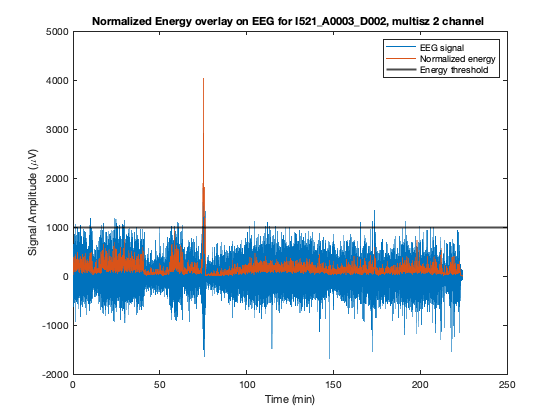
\includegraphics [width=5in]{jalp_hw3_15.png}

\end{enumerate}




\end{document}
    
